\documentclass{article}
\usepackage[utf8]{inputenc}
\usepackage{amsmath}
% \usepackage[linesnumbered,ruled,vlined]{algorithm2e}
% \usepackage{algorithmic}
\usepackage{cleveref}
\usepackage{titling}
\usepackage{flexisym}
\usepackage{enumitem}
\usepackage{color}
\usepackage{graphicx}
\usepackage{booktabs}
\usepackage{array}
\usepackage[paper=a4paper,margin=1in]{geometry}
\usepackage{scalerel,amssymb}
\usepackage{algorithm}
\usepackage{algpseudocode}
\usepackage{caption}
\usepackage{subcaption}
\usepackage{listings}
\usepackage{xspace}
\lstset{
  backgroundcolor=\color{backcolour},   
  commentstyle=\color{codegreen},
  keywordstyle=\color{magenta},
  language = Prolog,
  literate = {-}{-}1,
  breaklines=true, 
  numbers=left,
  basicstyle=\sffamily,
  %keywordstyle=\bfseries,
  %morekeywords={reached,  in, source, sink,edge,node},
}
\usepackage{xcolor}
\definecolor{codegreen}{rgb}{0,0.6,0}
\definecolor{codegray}{rgb}{0.5,0.5,0.5}
\definecolor{codepurple}{rgb}{0.58,0,0.82}
\definecolor{backcolour}{rgb}{0.95,0.95,0.92}
\usepackage{tikz}
\usepackage{scalerel,amssymb}
\usetikzlibrary{positioning, fit, calc, shapes.geometric}
\tikzset{block/.style={draw, thick, text width=2cm , minimum height=1.3cm, align=center},   
line/.style={-latex}     
} 
\algnewcommand\algorithmicforeach{\textbf{for each}}
\algdef{S}[FOR]{ForEach}[1]{\algorithmicforeach\ #1\ \algorithmicdo}
\def\mcirc{\mathbin{\scalerel*{\circ}{j}}}
\def\msquare{\mathord{\scalerel*{\Box}{gX}}}
\newtheorem{theorem}{Theorem}
\newtheorem{proposition}{Proposition}
\newtheorem{lemma}{Lemma}
\newtheorem{example}{Example}
\newtheorem{definition}{Definition}
\newtheorem{remark}{Remark}
\newtheorem{proof}{Proof}
\newcommand{\m}{\mathcal{M}}
\newcommand{\mzero}{\mathcal{M}_0}
\newcommand{\mone}{\mathcal{M}_1}
\newcommand{\program}[1]{\mathcal{P}(#1)}
\newcommand{\body}[1]{\mathsf{Body}(#1)}
\newcommand{\true}{\ensuremath{\mathsf{true}}\xspace}
\newcommand{\false}{\ensuremath{\mathsf{false}}\xspace}
\newcommand{\copyatom}[1]{#1\textprime}
\newcommand{\mmodel}[1]{\mathsf{MM}(#1)}
\newcommand{\Card}[1]{|#1|}
\newcommand{\Var}[1]{\mathsf{Var}(#1)}
\newcommand{\minimal}[1]{\mathsf{MM}(#1)}
\newcommand{\answer}[1]{\mathsf{AS}(#1)}
\title{Weekly Report}
\begin{document}
\date{13 March 2024}
\section{Methodology}
\begin{lstlisting}[caption={Program $\program{F}$},label={code:as_to_uc},captionpos=b,mathescape=true,escapechar=|,float]
  % for each variable X
  pos(X) $\vee$ neg(X) $\leftarrow$ v(X).|\label{line:each_variable}|
  % for each clause $C_i = \ell_1 \vee \ldots \ell_{k} \vee \neg{\ell_{k+1}} \vee \ldots \neg{\ell_{k+m}}$
  unsat $\leftarrow$ c(i), neg($\ell_1$), $\ldots$, neg($\ell_k$), pos($\ell_{k+1}$), $\ldots$, pos($\ell_{k+m}$).|\label{line:reach1}|
  % at least one clause must be falsified
  $\leftarrow$ not unsat.|\label{line:unsat}|
  % for each variable X
  pos(X) $\leftarrow$ unsat.
  neg(X) $\leftarrow$ unsat.
  % each c(i) is a free variable
  $\{$ c(i) $\}.$
\end{lstlisting}
\begin{lemma}
  Each answer set $\sigma \in \answer{\program{F}}$ one-to-one corresponds to an unsatisfiable core of $F$.
\end{lemma}
\begin{proof}
  The lemma has two parts to proof:
  \begin{enumerate}
    \item For each $\sigma \in \answer{\program{F}}$, $\sigma_{\downarrow c/1}$ corresponds to an unsatisfiable core of $F$
    \item Each unsatisfiable core $U$ of $F$ corresponds to an answer set of $\program{F}$ 
  \end{enumerate}
  Proof of `part $1$': For an answer set $\sigma \in \answer{\program{F}}$, let assume $\sigma_{\downarrow c/1} = \{c_{i_1}, \ldots, c_{i_k}\}$.
  We proof that the clause set of $\sigma_{\downarrow c/1}$ constitutes an unsatisfiable core of $F$.

  Under answer set semantics, unsat $\in \sigma$ (line~\ref{line:unsat} of encoding~\ref{code:as_to_uc}) and $\forall x \in \Var{F}$, $\{pos(x), neg(x)\} \subset \sigma$.
  Under clark completion semantics, since unsat $\in \sigma$, $\exists r \in \program{F}$ such that 
  $\body{r}$ is evaluated to $\true$. 
\end{proof}
\section{New MUS Solver using Clingo}
\section{Computing MUSes~\cite{LPMM2016} via Answer Set Programming}
\paragraph{Variables:}
\begin{itemize}
    \item For each clause $c$, introduce a variable $d(c)$
    \item For each variable $x$, introduce two variables $p(x)$ and $n(x)$
\end{itemize}
\paragraph{Rules:}
\begin{itemize}
    \item for each clause $\neg{\ell_1} \vee \ldots \vee 
    \neg{\ell_k} \vee \ell_{k+1} \vee \ldots \vee \ell_{k+m}$, 
    introduce a rule as follows:\\
    $u \leftarrow n(\ell_1), \ldots, n(\ell_k), p(\ell_{k+1}), p(\ell_{k+m}), d(c)$\\
    $u$ is true denotes that at least one of the clauses is satisfied.
    \item add a rule: $\leftarrow \textsf{not } u.$,
    which means that at least one of the clauses is unsatisfiable
    \item for each variable $x$, add a disjunctive rule: $p(x) ; n(x).$\\
    which denotes that each variable must be assigned to at least one of the values.
    \item for each variable $x$, add two rules: $p(x) \leftarrow u$ and $n(x) \leftarrow u$\\
    which denotes at least one of the clauses is UNSAT even after trying out all possible combinations of variables.
\end{itemize}
\paragraph{One-to-one correspondence between MUS and answer sets.}
Each of the $d(i)$-subset minimal models of the ASP program is a MUS of the original formula. 
\paragraph{Experimental Results}
\begin{table}[h]
  \centering
  \begin{tabular}{m{5em} m{5em} m{6em} m{10em}} 
  \toprule
  % & & \rotatebox{60}{\clingo} & \rotatebox{60}{DynASP} & \rotatebox{60}{Ganak}  & \rotatebox{60}{ApproxMC} & \rotatebox{60}{ApproxASP} \\ 
   & marco & unimus & Clingo\\
  \midrule
  %6491 & 6379 & 7743 & 5183 & 6094 & 5599\\
  \#Solved & 264 & 268 & 656\\
  \midrule
  PAR-$2$ & 5501 & 5480 & 2928\\
  \bottomrule
  \end{tabular}
  \caption{The performance of different MUS solvers.}
  \label{table:mus_counting_result}
\end{table}

\begin{figure}
  \centering
  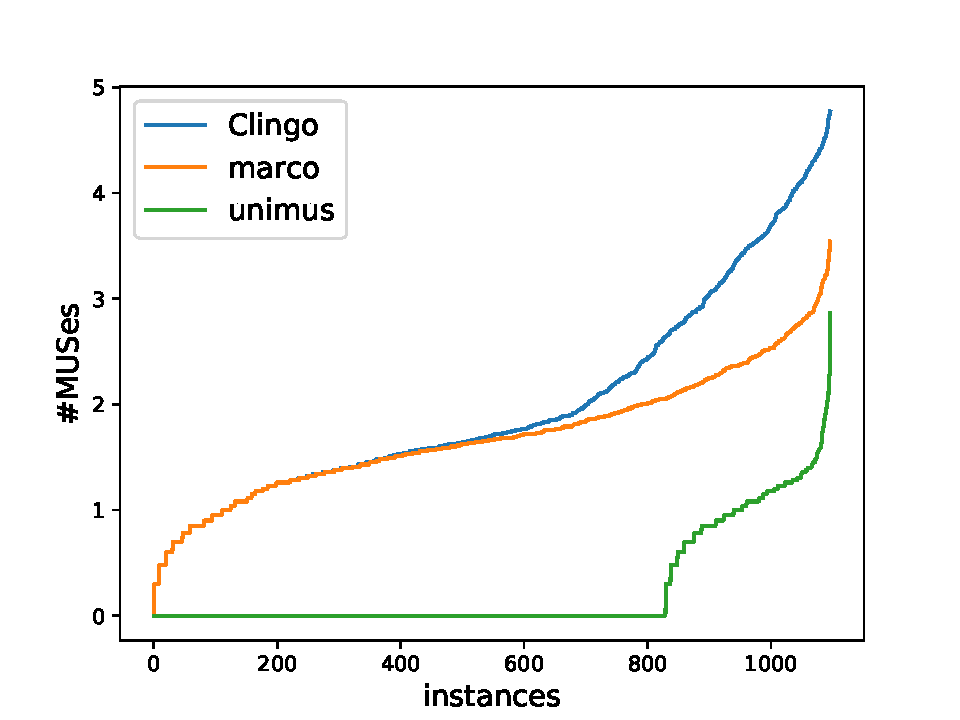
\includegraphics[scale=0.5]{images/countMUS.pdf}
  \caption{The number of enumerated MUSes by different MUS solvers.}
\end{figure}


\newpage
\section{Computing MUSes~\cite{LPMM2016} via Answer Set Programming}
\paragraph{Variables:}
\begin{itemize}
    \item For each clause $c$, introduce a variable $d(c)$
    \item For each variable $x$, introduce two variables $p(x)$ and $n(x)$
\end{itemize}
\paragraph{Rules:}
\begin{itemize}
    \item for each clause $\neg{\ell_1} \vee \ldots \vee 
    \neg{\ell_k} \vee \ell_{k+1} \vee \ldots \vee \ell_{k+m}$, 
    introduce a rule as follows:\\
    $u \leftarrow n(\ell_1), \ldots, n(\ell_k), p(\ell_{k+1}), p(\ell_{k+m}), d(c)$\\
    $u$ is true denotes that at least one of the clauses is satisfied.
    \item add a rule: $\leftarrow \textsf{not } u.$,
    which means that at least one of the clauses is unsatisfiable
    \item for each variable $x$, add a disjunctive rule: $p(x) ; n(x).$\\
    which denotes that each variable must be assigned to at least one of the values.
    \item for each variable $x$, add two rules: $p(x) \leftarrow u$ and $n(x) \leftarrow u$\\
    which denotes at least one of the clauses is UNSAT even after trying out all possible combinations of variables.
\end{itemize}
\paragraph{One-to-one correspondence between MUS and answer sets.}
Each of the $d(i)$-subset minimal models of the ASP program is a MUS of the original formula. 


\bibliography{main} 
\bibliographystyle{apalike}
\end{document}




